% wQFM-TREE-CPP: draft manuscript.
% Build: ./build.sh  (tectonic; package cache kept on the external SSD)
% Items marked \todo{...} need data, a decision or a check before submission.
\documentclass[11pt,a4paper]{article}

\usepackage[margin=2.5cm]{geometry}
\usepackage[T1]{fontenc}
\usepackage{lmodern}
\usepackage{microtype}
\usepackage{amsmath,amssymb}
\usepackage{booktabs}
\usepackage{multirow}
\usepackage{array}
\usepackage{xcolor}
\usepackage{tikz}
\usetikzlibrary{positioning,arrows.meta,calc,fit,backgrounds,decorations.pathreplacing}
\usepackage{pgfplots}
\pgfplotsset{compat=1.18}
\usepackage[numbers,sort&compress]{natbib}
\usepackage[hidelinks]{hyperref}
\usepackage{caption}
\usepackage{subcaption}
\captionsetup{font=small,labelfont=bf}
\setlength{\emergencystretch}{2em}

\newcommand{\todo}[1]{\textcolor{red}{[TODO: #1]}}
\newcommand{\wqfmtree}{wQFM-TREE}
\newcommand{\cpp}{wQFM-TREE-CPP}
\newcommand{\Oh}{\mathcal{O}}

% "before / now" paragraphs of the Methods
\definecolor{beforec}{RGB}{176,84,0}
\definecolor{nowc}{RGB}{0,84,160}
\definecolor{Ac}{RGB}{0,84,160}
\definecolor{Bc}{RGB}{196,96,0}
\definecolor{Xc}{RGB}{0,128,96}
\newcommand{\Before}{\par\smallskip\noindent\textbf{\textcolor{beforec}{Before (\wqfmtree).}}\ }
\newcommand{\Now}{\par\smallskip\noindent\textbf{\textcolor{nowc}{Now (\cpp).}}\ }
\newcommand{\Exact}{\par\smallskip\noindent\textbf{Why the result is unchanged.}\ }

% TikZ styles shared by the figures
\tikzset{
  arr/.style={-{Stealth[length=2mm]}, semithick},
  inner/.style={circle, fill=black, inner sep=1.1pt},
  tA/.style={inner sep=1.5pt, text=Ac, font=\small\bfseries},
  tB/.style={inner sep=1.5pt, text=Bc, font=\small\bfseries},
  tX/.style={inner sep=1.5pt, text=Xc, font=\small\bfseries},
  tleaf/.style={inner sep=1.5pt, font=\small},
  box/.style={draw, rounded corners=3pt, fill=gray!8, align=center, font=\small, inner sep=4pt},
}

\title{\cpp: exact, parallel and two orders of magnitude faster quartet-based species tree estimation from gene trees}
\author{Abdur Rafi\textsuperscript{1}\\[2pt]
\small\textsuperscript{1}Department of Computer Science and Engineering,\\
\small Bangladesh University of Engineering and Technology, Dhaka, Bangladesh\\[2pt]
\small\todo{co-authors, affiliations, corresponding author}}
\date{\todo{date}}

\begin{document}
\maketitle

\begin{abstract}
\noindent\textbf{Motivation:} \wqfmtree{} estimates species trees by running the weighted-quartet
Fiduccia--Mattheyses heuristic of wQFM directly on gene trees, without enumerating their
$\Theta(n^4)$ induced quartets. It is among the most accurate summary methods, but its Java
implementation needs hours on datasets with a thousand taxa and genes, and is slower than
ASTRAL and TREE-QMC on large inputs.

\noindent\textbf{Results:} We present \cpp, a reimplementation that performs the same search,
step for step, at a fraction of the cost. Each change is exact: it computes the same scores and gains
as before, only with less work. Node contributions at polytomies become closed forms (linear in the
degree instead of quadratic); each subproblem works on an exactly compressed copy of the gene trees,
derived from its parent's; the dummy taxa introduced by the divide-and-conquer cost only where they
occur; the candidates for the initial bipartition are scored together in one pass; and the search
runs in parallel with output that does not depend on the number of threads. Replaying the
decisions of the Java program shows that every score and gain agrees to within $10^{-11}$ (relative)
and that the trees are identical; across 1{,}101 ASTRAL-II runs the species trees are as accurate as
the published \wqfmtree{} trees. On the machine used for the published timings, with 200--1000 taxa
and 1000 genes and one thread like the published runs, \cpp{} is 45--90$\times$ faster than the Java
program, 27--47$\times$ faster than ASTRAL and 3.3--5.9$\times$ faster than TREE-QMC, and needs
7.6--18$\times$ less memory than the Java program. Eight threads, one per core, make it a further
4.7--6.4$\times$ faster: it analyses 1{,}000 taxa and 1{,}000 genes in $55\pm24$\,s instead of
12{,}275\,s, with the same trees as with any of 1 to 16 threads, and it
completes a replicate that the Java program could not finish in 48\,h in 51 minutes on one thread and
8 minutes on eight.

\noindent\textbf{Availability:} \url{https://github.com/abdur-rafi/wQFM-TREE-CPP}
\todo{license, archived release (Zenodo DOI)}
\end{abstract}

% =============================================================================================
\section{Introduction}

Species trees estimated from many loci must account for gene tree discordance, most prominently
from incomplete lineage sorting (ILS) \citep{maddison1997,degnan2009}. Summary methods first
estimate a tree per locus and then combine the gene trees. Quartet-based summary methods are
attractive because unrooted four-taxon gene trees have no anomaly zone; ASTRAL
\citep{mirarab2014astral,mirarab2015astral2,zhang2018astral3} is the most widely used. The
weighted-quartet heuristics wQMC \citep{avni2015wqmc} and wQFM \citep{mahbub2021wqfm} instead
amalgamate weighted quartets by divide and conquer, and wQFM has been shown to be as accurate as
ASTRAL or more. Their weakness is scalability: they enumerate and weight the $\Theta(n^4)$ quartets
induced by the gene trees.

TREE-QMC \citep{han2023treeqmc} removed this bottleneck for wQMC by computing the quartet graph
directly from the gene trees, and \wqfmtree{} \citep{rafi2025wqfmtree} did the same for wQFM: it
scores candidate bipartitions directly from the gene trees and obtains initial bipartitions from a
greedy consensus tree. \wqfmtree{} outperformed ASTRAL in 25 of 27 model conditions with 200--1000
taxa. Its Java implementation, however, needed 3.4\,h for 1000 taxa and 1000 genes, 5.5\,h for the
1KP green plant dataset (1{,}178 taxa, 410 genes), and could not finish one 1000-taxon replicate
with highly unresolved gene trees within 48\,h \citep{rafi2025wqfmtree}.

Here we show that the same search can be carried out more than two orders of magnitude faster.
\cpp{} is a reimplementation in C++20 that makes the same decisions as the Java program but
reorganises the computation behind each of them. Figure~\ref{fig:map} shows where in the search
each change acts and Table~\ref{tab:summary} summarises them; Section~\ref{sec:methods} explains
each one against what the Java program did, with examples. Our contributions are:
\begin{itemize}
\item a \emph{unit formulation} in which real taxa and the dummy taxa of the divide-and-conquer are
  weighted units, and closed-form node contributions that make a polytomy of degree $D$ cost
  $\Oh(D)$ instead of $\Oh(D^2)$ (Sections~\ref{sec:units}--\ref{sec:closed});
\item exact \emph{compression} of each subproblem's gene trees, derived from the parent
  subproblem's compressed trees (Section~\ref{sec:compress});
\item a \emph{sparse treatment of dummy taxa}, whose cost does not grow with the number of dummy
  taxa in a subproblem (Section~\ref{sec:dummies});
\item \emph{search-level} changes that keep the search unchanged: batched scoring of the
  initial-bipartition candidates and deferred, parallel application of moves
  (Sections~\ref{sec:gains} and~\ref{sec:initial});
\item \emph{deterministic parallelism}: results are byte-identical for any number of threads
  (Section~\ref{sec:parallel});
\item a \emph{validation methodology} that compares every score and gain with brute-force quartet
  enumeration and with step-by-step replays of the Java program (Section~\ref{sec:validation}).
\end{itemize}

% =============================================================================================
\section{Background: \wqfmtree}\label{sec:background}

\paragraph{Divide and conquer.} Given gene trees $\mathcal{G}=\{g_1,\dots,g_k\}$ on $n$ taxa, wQFM
\citep{reaz2014qfm,mahbub2021wqfm} splits the taxa into a bipartition $(A,B)$, solves the two
sides recursively and joins the two subtrees (Figure~\ref{fig:dc}). So that each side still knows
where the rest of the taxa are, it receives a \emph{dummy taxon} standing for the other side. Later
subproblems therefore contain real taxa and dummy taxa; a dummy taxon may contain earlier dummy
taxa, and the real taxa under a dummy taxon receive fractional weights that add up to one (Eq.~1
of \citep{rafi2025wqfmtree}). We call real and dummy taxa together the \emph{units} of a
subproblem. A subproblem with at most three units is a star, and the recursion stops.

\begin{figure}[t]
\centering
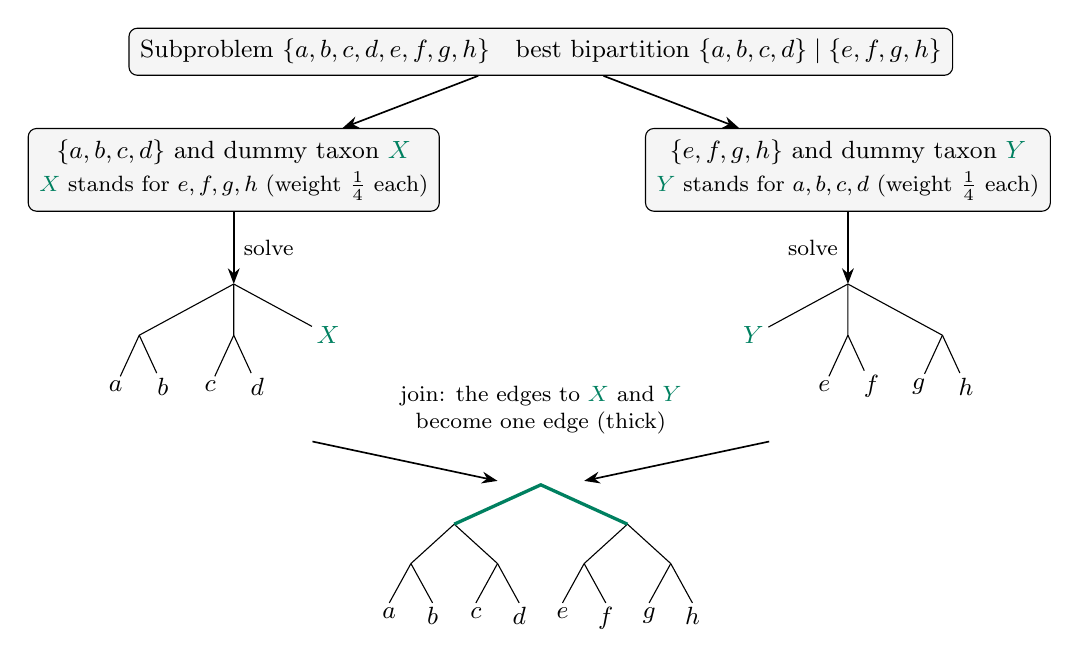
\begin{tikzpicture}[level distance=6.5mm]
\node[box] (top) at (0,0) {Subproblem $\{a,b,c,d,e,f,g,h\}$\quad best bipartition $\{a,b,c,d\}\mid\{e,f,g,h\}$};
\node[box] (L) at (-3.9,-1.5) {$\{a,b,c,d\}$ and dummy taxon \textcolor{Xc}{$X$}\\[1pt]
  \footnotesize \textcolor{Xc}{$X$} stands for $e,f,g,h$ (weight $\tfrac14$ each)};
\node[box] (R) at (3.9,-1.5) {$\{e,f,g,h\}$ and dummy taxon \textcolor{Xc}{$Y$}\\[1pt]
  \footnotesize \textcolor{Xc}{$Y$} stands for $a,b,c,d$ (weight $\tfrac14$ each)};
\draw[arr] (top) -- (L); \draw[arr] (top) -- (R);
\begin{scope}[shift={(-3.9,-2.95)}, level 1/.style={sibling distance=12mm}, level 2/.style={sibling distance=6mm}]
\coordinate (t1) child {coordinate child {node[tleaf]{$a$}} child {node[tleaf]{$b$}}}
  child {coordinate child {node[tleaf]{$c$}} child {node[tleaf]{$d$}}}
  child {node[tX]{$X$}};
\end{scope}
\begin{scope}[shift={(3.9,-2.95)}, level 1/.style={sibling distance=12mm}, level 2/.style={sibling distance=6mm}]
\coordinate (t2) child {node[tX]{$Y$}}
  child {coordinate child {node[tleaf]{$e$}} child {node[tleaf]{$f$}}}
  child {coordinate child {node[tleaf]{$g$}} child {node[tleaf]{$h$}}};
\end{scope}
\draw[arr] (L.south) -- node[right, font=\footnotesize]{solve} (t1);
\draw[arr] (R.south) -- node[left, font=\footnotesize]{solve} (t2);
\draw[arr] (-2.9,-4.95) -- (-0.55,-5.45);
\draw[arr] (2.9,-4.95) -- (0.55,-5.45);
\node[font=\footnotesize, align=center] at (0,-4.55) {join: the edges to \textcolor{Xc}{$X$} and \textcolor{Xc}{$Y$}\\ become one edge (thick)};
\coordinate (jroot) at (0.000,-5.500);
\coordinate (jl) at (-1.100,-6.000);
\coordinate (Jn3) at (-1.650,-6.500);
\coordinate (JLa) at (-1.925,-7.000);
\node[tleaf, below] at (JLa) {$a$};
\draw (Jn3) -- (JLa);
\coordinate (JLb) at (-1.375,-7.000);
\node[tleaf, below] at (JLb) {$b$};
\draw (Jn3) -- (JLb);
\draw (jl) -- (Jn3);
\coordinate (Jn4) at (-0.550,-6.500);
\coordinate (JLc) at (-0.825,-7.000);
\node[tleaf, below] at (JLc) {$c$};
\draw (Jn4) -- (JLc);
\coordinate (JLd) at (-0.275,-7.000);
\node[tleaf, below] at (JLd) {$d$};
\draw (Jn4) -- (JLd);
\draw (jl) -- (Jn4);
\draw (jroot) -- (jl);
\coordinate (jr) at (1.100,-6.000);
\coordinate (Jn6) at (0.550,-6.500);
\coordinate (JLe) at (0.275,-7.000);
\node[tleaf, below] at (JLe) {$e$};
\draw (Jn6) -- (JLe);
\coordinate (JLf) at (0.825,-7.000);
\node[tleaf, below] at (JLf) {$f$};
\draw (Jn6) -- (JLf);
\draw (jr) -- (Jn6);
\coordinate (Jn7) at (1.650,-6.500);
\coordinate (JLg) at (1.375,-7.000);
\node[tleaf, below] at (JLg) {$g$};
\draw (Jn7) -- (JLg);
\coordinate (JLh) at (1.925,-7.000);
\node[tleaf, below] at (JLh) {$h$};
\draw (Jn7) -- (JLh);
\draw (jr) -- (Jn7);
\draw (jroot) -- (jr);
\draw[very thick, Xc] (jl) -- (jroot) -- (jr);
\end{tikzpicture}
\caption{The divide-and-conquer of wQFM on eight taxa. After the best bipartition is found, each
side becomes a subproblem with one more unit, a dummy taxon for the other side, whose real taxa
share a total weight of one. The solved subtrees are joined through the dummy taxa (thick edge).
Deeper subproblems can contain several dummy taxa, nested in one another.}
\label{fig:dc}
\end{figure}

\paragraph{Search for a bipartition.} Within a subproblem, a bipartition is found in two steps.
The \emph{initial bipartition} is the best-scoring one among those induced by the edges of a
greedy consensus tree of the gene trees. It is then improved by Fiduccia--Mattheyses (FM) passes
\citep{fiduccia1982}: units are moved to the other side one at a time, always the unlocked unit with
the largest \emph{gain} (the change of the score if it moves), until no unit can move; the best prefix
of the pass is kept, and passes repeat (at most six) while they improve the score. Every move
changes every unit's gain, so all gains are recomputed after each move.

\paragraph{Score.} For a bipartition $(A,B)$, a quartet with two taxa on each side, say
$\{a_1,a_2\}\subseteq A$ and $\{b_1,b_2\}\subseteq B$, is \emph{satisfied} by a gene tree if the
gene tree shows $a_1a_2\mid b_1b_2$, \emph{violated} if it shows one of the other two topologies,
and \emph{unresolved} if the four taxa meet at a polytomy. The score of $(A,B)$ is the total weight
of satisfied minus violated quartets over all gene trees; a quartet's weight is the product of its
taxa's weights, and quartets with two taxa under the same dummy taxon are excluded. \wqfmtree{}
computes it without listing quartets: every satisfied or unresolved quartet is counted at one
internal node of the gene tree, which gives
\begin{equation}\label{eq:score}
  \mathrm{Score}(A,B,\mathcal{G}) \;=\; \sum_{g\in\mathcal{G}}
  \Bigl( 2\sum_{u\in g} f_u \;-\; w(P_A(g))\,w(P_B(g)) \Bigr),
  \qquad f_u = w(S(g,u)) + \tfrac12 w(U(g,u)),
\end{equation}
where $S(g,u)$ and $U(g,u)$ are the satisfied and unresolved quartets counted at node $u$, and
$w(P_A(g))\,w(P_B(g))$ is the weight of all quartets with two taxa on each side
\citep{rafi2025wqfmtree}. Eq.~\eqref{eq:score} is ``satisfied minus violated'' rewritten with
$\text{violated}=\text{all}-\text{satisfied}-\text{unresolved}$. Example~1 below computes it on a
small tree.

Table~\ref{tab:notation} collects the notation used in the rest of the paper.

\begin{table}[t]
\centering\small
\caption{Notation.}
\label{tab:notation}
\begin{tabular}{@{}ll@{}}
\toprule
$n$, $k$ & number of taxa, number of gene trees \\
$(A,B)$ & the current bipartition of a subproblem's units (real and dummy taxa) \\
$s$, $d$ & number of units and of dummy taxa in a subproblem \\
$u$, $D$ & an internal node of a gene tree and its degree (number of branches around it) \\
$a_i$, $b_i$ & total weight of the units of $A$, of $B$, in branch $i$ of $u$ \\
$\rho_i$ & number of real taxa of $B$ in branch $i$ \\
$x_{ki}$ & weight of dummy taxon $k$ in branch $i$; $X_k$ its weight in the whole gene tree \\
$PA_{ij}$, $PB_i$ & weight of pairs of $A$ split between branches $i$ and $j$; of pairs of $B$ inside branch $i$ \\
$f_u$ & contribution of node $u$ to the score, Eq.~\eqref{eq:score} \\
$N$ & total number of nodes of all gene trees \\
$N_s$ & number of nodes of a subproblem's compressed gene trees (Section~\ref{sec:compress}) \\
\bottomrule
\end{tabular}
\end{table}

% =============================================================================================
\section{Methods}\label{sec:methods}

\subsection{Overview of the changes}\label{sec:overview}

\cpp{} keeps every decision of the Java program (Section~\ref{sec:faithful}); it changes how much
work each decision costs. Figure~\ref{fig:map} places each change in the search and
Table~\ref{tab:summary} compares the costs. Nearly all of the running time goes into passes over
the gene trees of a subproblem: one per FM move and, in the Java program, one per candidate initial
bipartition (about half of its time). Most of our changes make such a pass cheaper, by shrinking the
trees it visits (compression), the work per node (closed forms, sparse dummy taxa) or the wall time
(parallel chunks); the batched candidates also need fewer passes.

\begin{figure}[t]
\centering
\begin{tikzpicture}[
  stage/.style={draw, rounded corners=3pt, fill=gray!8, align=center, font=\small, text width=3.5cm, minimum height=8mm},
  note/.style={font=\footnotesize, align=left, text width=8.3cm, anchor=west}]
\node[stage] (gt) {Gene trees};
\node[stage, below=4mm of gt] (cons) {Greedy consensus tree};
\node[stage, below=9mm of cons] (setup) {Set up the gene trees of the subproblem};
\node[stage, below=4mm of setup] (init) {Initial bipartition};
\node[stage, below=4mm of init] (fm) {FM passes\\(score and gains after every move)};
\node[stage, below=4mm of fm] (div) {Divide: one dummy taxon per side};
\node[stage, below=9mm of div] (join) {Join the subtrees};
\node[stage, below=4mm of join] (sp) {Species tree};
\foreach \x/\y in {gt/cons, cons/setup, setup/init, init/fm, fm/div, div/join, join/sp} \draw[arr] (\x) -- (\y);
\draw[arr, dashed] (div.west) -- ++(-5mm,0) |- node[pos=0.25, left, font=\footnotesize, align=right]{two child\\subproblems} (setup.west);
\begin{scope}[on background layer]
\node[draw=gray, dashed, rounded corners, fit=(setup)(div), inner sep=2.5mm,
  label={[font=\footnotesize, anchor=south east, inner sep=1pt, xshift=-3mm]north:for every subproblem}] {};
\end{scope}
\node[note] at ($(setup.east)+(7mm,0)$) {\textbf{Compressed} trees, derived from the parent's (\S\ref{sec:compress})};
\node[note] at ($(init.east)+(7mm,0)$) {All candidates \textbf{scored together} in one pass (\S\ref{sec:initial})};
\node[note] at ($(fm.east)+(7mm,0)$) {\textbf{Closed forms}: $\Oh(D)$ per polytomy (\S\ref{sec:closed}); \textbf{sparse dummy taxa} (\S\ref{sec:dummies}); \textbf{deferred moves}, gene trees in \textbf{parallel chunks} (\S\ref{sec:gains}, \S\ref{sec:parallel})};
\node[note] at ($(div.east)+(7mm,0)$) {The two children run \textbf{concurrently} (\S\ref{sec:parallel})};
\node[note] at ($(cons.east)+(7mm,0)$) {Built in, without PAUP; a given consensus tree can still be used};
\end{tikzpicture}
\caption{The \wqfmtree{} search and where \cpp{} changes it. Every box does the same as in the Java
program; the notes on the right name what \cpp{} does differently, with the section that explains it.}
\label{fig:map}
\end{figure}

\begin{table}[t]
\centering\footnotesize
\caption{What changes, per part of the search. Costs are per FM move in a subproblem with $s$ units,
$d$ of them dummy taxa, on gene trees with $N$ nodes in total; $D$ is the degree of a polytomy,
$N_s\approx N s/n$ the size of the compressed trees and $L$ the total length of the per-node dummy
lists (Section~\ref{sec:dummies}). The search, and therefore the output, is the same.}
\label{tab:summary}
\setlength{\tabcolsep}{4pt}
\begin{tabular}{@{}>{\raggedright}p{2.5cm}>{\raggedright}p{4.6cm}>{\raggedright}p{4.6cm}>{\raggedright\arraybackslash}p{2.6cm}@{}}
\toprule
Part & Before: \wqfmtree{} (Java) & Now: \cpp & Cost per move \\
\midrule
Gene trees of a subproblem & all gene trees, in full, at every level of the recursion & compressed for the subproblem, computed from the parent's compressed trees (\S\ref{sec:compress}) & $N \to N_s$ \\ \addlinespace[3pt]
Node contribution & double sums over pairs of branches & closed forms in eleven power sums (\S\ref{sec:closed}) & $\Oh(D^2)\to\Oh(D)$ per polytomy \\ \addlinespace[3pt]
Dummy taxa & an array of length $d$ on every branch of every node & lists at the nodes where a dummy taxon occurs, one polynomial per tree for the rest (\S\ref{sec:dummies}) & $\Oh(Nd)\to\Oh(N_s+L)$ \\ \addlinespace[3pt]
All gains of a tree & one bottom-up and one top-down pass (kept) & the same two passes; moves applied inside the next pass (\S\ref{sec:gains}) & linear in both \\ \addlinespace[3pt]
Initial bipartition & each consensus candidate set up and scored separately & candidates described by the taxa that move; all scored in one pass (\S\ref{sec:initial}) & --- \\ \addlinespace[3pt]
Repeated nodes & identical tripartitions evaluated once (global table, string keys) & identical rooted subtrees evaluated once per chunk of trees (\S\ref{sec:shared}, preliminary) & --- \\ \addlinespace[3pt]
Threads & one & chunks of gene trees and sibling subproblems in parallel; same output for any thread count (\S\ref{sec:parallel}) & --- \\ \addlinespace[3pt]
Storage & objects, per-branch arrays, string keys & flat arrays of 32-bit integers and doubles & 7.6--18$\times$ less memory \\
\bottomrule
\end{tabular}
\end{table}

% ---------------------------------------------------------------------------------------------
\subsection{Units and what a node contributes}\label{sec:units}

Removing an internal node $u$ of degree $D$ splits a gene tree into $D$ branches: one per child, and
the \emph{top branch} (the rest of the tree). Everything $u$ contributes to the score depends only
on how much of $A$ and of $B$ lies in each branch. For branch $i$ let $a_i$ and $b_i$ be the total
weight of the units of $A$ and of $B$ in it. The pairs that matter are pairs of $A$ split between
two branches and pairs of $B$ inside one branch; leaving out pairs under the same dummy taxon,
their weights are
\begin{equation}\label{eq:pairs}
  PA_{ij} = a_i a_j - \sum_{k\in A} x_{ki}x_{kj}, \qquad
  PB_{i} = \tfrac12\Bigl(b_i^2 - \rho_i - \sum_{k\in B} x_{ki}^2\Bigr),
\end{equation}
where the sums run over the dummy taxa on each side and $\rho_i$ removes the pairs of a real taxon
with itself (weight one). A quartet $a_1a_2\mid b_1b_2$ is satisfied and counted at $u$ when $a_1$
and $a_2$ are in different branches $i\neq j$ and $b_1,b_2$ together in a third branch $l$; it is
unresolved at a polytomy when $b_1,b_2$ are in two further, different branches. Hence
\begin{equation}\label{eq:SU}
  w(S(g,u)) = \sum_{i<j} PA_{ij}\sum_{l\neq i,j} PB_l, \qquad
  w(U(g,u)) = \sum_{i<j} PA_{ij}\sum_{\substack{l<m\\ l,m\notin\{i,j\}}} PB_{lm},
\end{equation}
with $PB_{lm}=b_lb_m-\sum_{k\in B}x_{kl}x_{km}$. A binary node has three branches (children $0$ and
$1$, top branch $2$), no unresolved quartets, and
\begin{equation}\label{eq:binary}
  f_u = PA_{01}PB_2 + PA_{12}PB_0 + PA_{20}PB_1 .
\end{equation}
\cpp{} stores at each node only the totals of its subtree; the top branch's values follow by
subtracting them from the totals of the whole gene tree.

\begin{figure}[t]
\centering
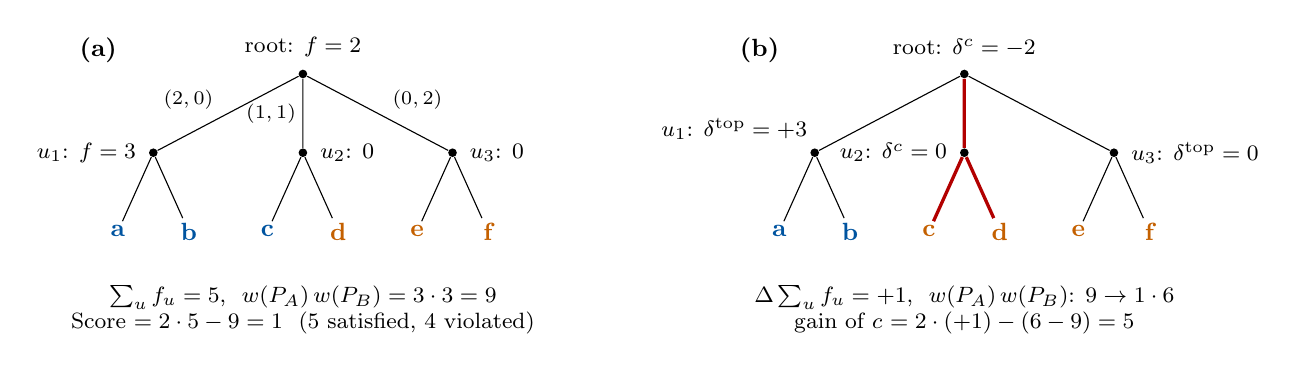
\begin{tikzpicture}[level distance=10mm, level 1/.style={sibling distance=19mm}, level 2/.style={sibling distance=9mm}]
\begin{scope}
\node[inner] (r) {}
  child {node[inner] (u1) {} child {node[tA]{a}} child {node[tA]{b}}}
  child {node[inner] (u2) {} child {node[tA]{c}} child {node[tB]{d}}}
  child {node[inner] (u3) {} child {node[tB]{e}} child {node[tB]{f}}};
\node[above=1pt of r, font=\footnotesize] {root: $f=2$};
\node[left=1pt of u1, font=\footnotesize] {$u_1$: $f=3$};
\node[right=1pt of u2, font=\footnotesize] {$u_2$: $0$};
\node[right=1pt of u3, font=\footnotesize] {$u_3$: $0$};
\path (r) -- (u1) node[pos=0.55, above left=-1pt, font=\scriptsize] {$(2,0)$};
\path (r) -- (u2) node[pos=0.5, left=-1pt, font=\scriptsize] {$(1,1)$};
\path (r) -- (u3) node[pos=0.55, above right=-1pt, font=\scriptsize] {$(0,2)$};
\node[font=\footnotesize, align=center] at (0,-3.0) {$\sum_u f_u=5$, \ $w(P_A)\,w(P_B)=3\cdot3=9$\\ Score $=2\cdot5-9=1$ \ (5 satisfied, 4 violated)};
\node[font=\small\bfseries] at (-2.6,0.3) {(a)};
\end{scope}
\begin{scope}[xshift=8.4cm]
\node[inner] (r) {}
  child {node[inner] (u1) {} child {node[tA]{a}} child {node[tA]{b}}}
  child[edge from parent/.style={draw, very thick, red!70!black}] {node[inner] (u2) {}
      child {node[tB]{c}} child[edge from parent/.style={draw}] {node[tB]{d}}}
  child {node[inner] (u3) {} child {node[tB]{e}} child {node[tB]{f}}};
\node[above=1pt of r, font=\footnotesize] {root: $\delta^{c}=-2$};
\node[above left=0pt and -2pt of u1, font=\footnotesize] {$u_1$: $\delta^{\mathrm{top}}=+3$};
\node[left=1pt of u2, font=\footnotesize] {$u_2$: $\delta^{c}=0$};
\node[right=1pt of u3, font=\footnotesize] {$u_3$: $\delta^{\mathrm{top}}=0$};
\node[font=\footnotesize, align=center] at (0,-3.0) {$\Delta\sum_u f_u=+1$, \ $w(P_A)\,w(P_B)$: $9\to1\cdot6$\\ gain of $c$ $=2\cdot(+1)-(6-9)=5$};
\node[font=\small\bfseries] at (-2.6,0.3) {(b)};
\end{scope}
\end{tikzpicture}
\caption{Example~1. (a) Gene tree $((a,b),(c,d),(e,f))$ and the bipartition
$A=\{\textcolor{Ac}{a,b,c}\}$, $B=\{\textcolor{Bc}{d,e,f}\}$, with each node's contribution $f_u$;
the root's branches are labelled with $(a_i,b_i)$. (b) Moving $c$ to $B$. Nodes off the path from
$c$ to the root (red) see $c$ change sides in their top branch; nodes on the path see it in the
child branch that leads to $c$. The values are the changes of $f_u$.}
\label{fig:example}
\end{figure}

\paragraph{Example 1.} In the gene tree of Figure~\ref{fig:example}a, with $A=\{a,b,c\}$ and
$B=\{d,e,f\}$, there are $3\cdot3=9$ quartets with two taxa on each side. At $u_1$ the branches are
$\{a\}$, $\{b\}$ and the rest $\{c,d,e,f\}$, so $PA_{01}=1\cdot1$ and $PB_2=\binom32=3$: $f_{u_1}=3$,
the satisfied quartets $ab\mid de$, $ab\mid df$, $ab\mid ef$. At the root, $PA_{01}=2\cdot1$ (pairs
$ac$, $bc$) and $PB_2=\binom22=1$ (pair $ef$): $f=2$. Nodes $u_2$ and $u_3$ contribute nothing, so
$\sum_u f_u=5$ and Score $=2\cdot5-9=1$: five quartets are satisfied and the four quartets
$ac\mid de$, $ac\mid df$, $bc\mid de$, $bc\mid df$ are violated.

% ---------------------------------------------------------------------------------------------
\subsection{Polytomies in time linear in their degree}\label{sec:closed}

\Before Eq.~\eqref{eq:SU} is a double sum over pairs of branches. Evaluated as written, a node of
degree $D$ costs $\Oh(D^2)$ for $w(S)$, and the gains of its units cost the same again. Gene trees
estimated from short alignments often contain large polytomies: the 1KP gene trees have 24{,}417
polytomy nodes with up to 576 branches.

\Now The double sums are rewritten in terms of sums over single branches. For $w(S)$ without dummy
taxa, write $A=\sum_ia_i$, $p_i=PB_i=\binom{b_i}{2}$, $P=\sum_ip_i$ and
$E_A=\sum_{i<j}a_ia_j=(A^2-\sum_ia_i^2)/2$. The inner sum of Eq.~\eqref{eq:SU} is
$P-p_i-p_j$, so
\begin{equation}\label{eq:S-closed}
  w(S(g,u)) = \sum_{i<j}a_ia_j\,(P-p_i-p_j)
  = P\,E_A - A\sum_i a_ip_i + \sum_i a_i^2p_i ,
\end{equation}
using $\sum_{i<j}a_ia_j(p_i+p_j)=\sum_{i}a_ip_i(A-a_i)$. The same inclusion--exclusion turns
$w(U(g,u))$ into products of the sums $\sum_ia_ib_i$, $\sum_ia_ib_i^2$, $\sum_ia_i^2b_i$ and
$\sum_ia_i^2b_i^2$ with $A$, $B$, $E_A$ and $E_B$:
\begin{equation}\label{eq:U-closed}
\begin{split}
  w(U(g,u)) = E_AE_B &- A\Bigl(B\sum_i a_ib_i - \sum_i a_ib_i^2\Bigr)
     + \Bigl(B\sum_i a_i^2b_i - \sum_i a_i^2b_i^2\Bigr)\\
     &+ \tfrac12\Bigl(\bigl(\sum_i a_ib_i\bigr)^2 - \sum_i a_i^2b_i^2\Bigr).
\end{split}
\end{equation}
Eleven sums over the branches determine $f_u$, so a node costs $\Oh(D)$. Moving a unit changes the
values of one branch: subtracting its old terms from the sums and adding the new ones gives the new
$f_u$ in $\Oh(1)$, and with it the unit's gain at this node. Dummy taxa add correction terms of the
same kind (Appendix~\ref{app:poly}).

\Exact The closed forms are algebraic identities: they compute the same numbers as the double
sums. On the top level of the 1KP data the closed-form scores and gains agreed bit for bit with the
Java program.

\paragraph{Example 2.} A polytomy with four branches holding $(a_i,b_i)=(2,0),(1,1),(0,2),(1,1)$.
The double sums of Eq.~\eqref{eq:SU} run over the $6$ pairs of branches and give $w(S)=5$ and
$w(U)=8$. With the sums $A=B=4$, $E_A=E_B=5$, $P=1$, $\sum a_ip_i=\sum a_i^2p_i=0$
and $\sum a_ib_i=\sum a_ib_i^2=\sum a_i^2b_i=\sum a_i^2b_i^2=2$, Eq.~\eqref{eq:S-closed} gives
$w(S)=1\cdot5=5$ and Eq.~\eqref{eq:U-closed} gives $w(U)=25-4(8-2)+(8-2)+\tfrac12(4-2)=8$, so
$f_u=5+8/2=9$. For the largest 1KP polytomy ($D=576$), the double sums run over 165{,}600 pairs of
branches; the closed forms over its 576 branches.

% ---------------------------------------------------------------------------------------------
\subsection{All gains of a gene tree in two passes}\label{sec:gains}

\Before \wqfmtree{} already computes the gains of all real taxa of a gene tree in two passes
(Figure~\ref{fig:example}b). When a real taxon $t$ changes sides, a node $u$ sees the change in one
branch only: in the child branch that leads to $t$ if $u$ is an ancestor of $t$, and in its top
branch otherwise. Write $\delta^{\mathrm{top}}_u$ and $\delta^c_u$ for the change of $f_u$ in the
two cases; they depend on $t$ only through its side, because every real taxon has weight one. The
gain of $t$ in tree $g$ is then
\begin{equation}\label{eq:gain}
  \mathrm{gain}_g(t) = 2\Bigl(\underbrace{\textstyle\sum_{u}\delta^{\mathrm{top}}_u}_{\text{same for every } t}
     + \sum_{(u,c)\,\in\,\mathrm{path}(t)}\bigl(\delta^{c}_u-\delta^{\mathrm{top}}_u\bigr)\Bigr)
     - \Delta\bigl(w(P_A)\,w(P_B)\bigr),
\end{equation}
where the path runs from the root to $t$'s leaf through child $c$ at each node $u$. A bottom-up pass
computes every node's $\delta$ values and pushes the differences
$\delta^c_u-\delta^{\mathrm{top}}_u$ to the children; a top-down pass adds them up along every path.
The Java program stores two such values per branch (for a taxon of $A$ and one of $B$), and one
value per dummy taxon per branch for the dummy gains.

\Now We keep the two passes. What changes is the cost per node: $\delta^{\mathrm{top}}_u$ and every
$\delta^c_u$ come from the closed forms of Section~\ref{sec:closed} in $\Oh(1)$ per branch, and the
dummy gains no longer need per-branch arrays (Section~\ref{sec:dummies}). We also no longer apply a
move as a separate pass over the gene trees: a move only records itself, and the next pass applies it
to each chunk of gene trees just before scoring the chunk (Section~\ref{sec:parallel}), so the update
runs in parallel and needs no synchronisation of its own.

\paragraph{Example 1, continued.} Moving $c$ to $B$ (Figure~\ref{fig:example}b) changes $f$ by
$+3$ at $u_1$ (its top branch now holds $\binom42=6$ pairs of $B$ instead of 3), by $0$ at $u_3$
and $u_2$, and by $-2$ at the root. The pairs across the sides fall from $3\cdot3$ to $1\cdot6$, so the
gain is $2\cdot(+1)+3=5$: the new score is $6$, all six quartets $ab\mid\cdot\cdot$ being satisfied.

% ---------------------------------------------------------------------------------------------
\subsection{Compressed gene trees per subproblem}\label{sec:compress}

\Before Every subproblem, however small, is scored on all gene trees in full. A subproblem with $s$
units still visits all $N$ nodes per FM move, so each level of the recursion costs about as much as
the top level.

\Now Consider a node whose branches, apart from one, all contain only taxa of a single dummy taxon
$X$. Any quartet counted at it has two taxa under $X$, and such quartets are excluded from the
score; the node contributes nothing. In each subproblem we therefore collapse every maximal part of
a gene tree whose units all belong to one dummy taxon into a single leaf carrying their total weight
(Figure~\ref{fig:compress}). ``Maximal'' is judged on the unrooted tree: a part above a node, not
only a subtree below it, can belong to one dummy taxon. Sibling leaves of the same dummy taxon are
merged, and gene trees left with fewer than four units are dropped. A compressed tree keeps roughly
a fraction $s/n$ of the nodes, so after compression the top levels of the recursion dominate.

A child subproblem's units are unions of its parent's units, so its compressed trees can be computed
from the parent's compressed trees instead of from the full gene trees. On the 1KP data this cut
the setup time of all subproblems from 15.8\,s to 0.8\,s.

\Exact Only nodes that contribute nothing are removed, and the collapsed leaves keep the weights
that the remaining nodes see. Brute-force enumeration confirms that scores and gains are unchanged
(Section~\ref{sec:validation}). In instrumented Java runs, the compressed trees would need 3.9--4.9$\times$
fewer node visits during FM, and 4.4--5.2$\times$ fewer for the initial bipartitions, on simulated and
1KP data.

\begin{figure}[t]
\centering
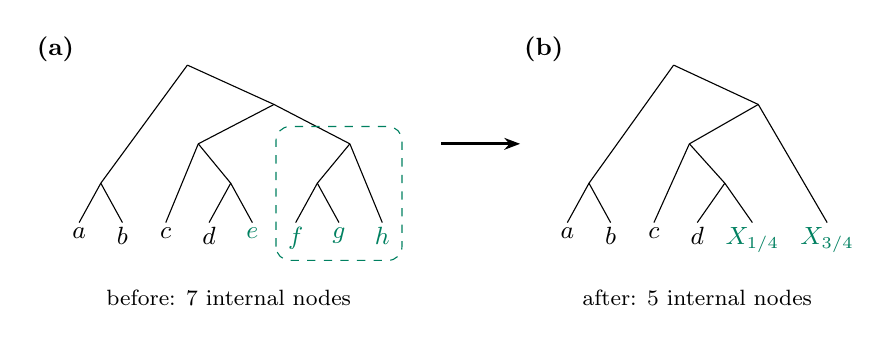
\begin{tikzpicture}
\coordinate (Cn1) at (1.375,2.000);
\coordinate (Cn2) at (0.275,0.500);
\coordinate (CLa) at (0.000,0.000);
\node[tleaf, below] at (CLa) {$a$};
\draw (Cn2) -- (CLa);
\coordinate (CLb) at (0.550,0.000);
\node[tleaf, below] at (CLb) {$b$};
\draw (Cn2) -- (CLb);
\draw (Cn1) -- (Cn2);
\coordinate (Cn3) at (2.475,1.500);
\coordinate (Cn4) at (1.513,1.000);
\coordinate (CLc) at (1.100,0.000);
\node[tleaf, below] at (CLc) {$c$};
\draw (Cn4) -- (CLc);
\coordinate (Cn5) at (1.925,0.500);
\coordinate (CLd) at (1.650,0.000);
\node[tleaf, below] at (CLd) {$d$};
\draw (Cn5) -- (CLd);
\coordinate (CLe) at (2.200,0.000);
\node[tX, below] at (CLe) {$e$};
\draw (Cn5) -- (CLe);
\draw (Cn4) -- (Cn5);
\draw (Cn3) -- (Cn4);
\coordinate (kk) at (3.438,1.000);
\coordinate (Cn7) at (3.025,0.500);
\coordinate (CLf) at (2.750,0.000);
\node[tX, below] at (CLf) {$f$};
\draw (Cn7) -- (CLf);
\coordinate (CLg) at (3.300,0.000);
\node[tX, below] at (CLg) {$g$};
\draw (Cn7) -- (CLg);
\draw (kk) -- (Cn7);
\coordinate (CLh) at (3.850,0.000);
\node[tX, below] at (CLh) {$h$};
\draw (kk) -- (CLh);
\draw (Cn3) -- (kk);
\draw (Cn1) -- (Cn3);
\draw[Xc, dashed, rounded corners=5pt] (2.5,-0.48) rectangle (4.1,1.22);
\node[font=\footnotesize] at (1.9,-0.95) {before: 7 internal nodes};
\node[font=\small\bfseries] at (-0.3,2.2) {(a)};
\draw[arr, very thick] (4.6,1.0) -- (5.6,1.0);
\coordinate (Dn1) at (7.550,2.000);
\coordinate (Dn2) at (6.475,0.500);
\coordinate (DLa) at (6.200,0.000);
\node[tleaf, below] at (DLa) {$a$};
\draw (Dn2) -- (DLa);
\coordinate (DLb) at (6.750,0.000);
\node[tleaf, below] at (DLb) {$b$};
\draw (Dn2) -- (DLb);
\draw (Dn1) -- (Dn2);
\coordinate (Dn3) at (8.625,1.500);
\coordinate (Dn4) at (7.750,1.000);
\coordinate (DLc) at (7.300,0.000);
\node[tleaf, below] at (DLc) {$c$};
\draw (Dn4) -- (DLc);
\coordinate (Dn5) at (8.200,0.500);
\coordinate (DLd) at (7.850,0.000);
\node[tleaf, below] at (DLd) {$d$};
\draw (Dn5) -- (DLd);
\coordinate (DLX14) at (8.550,0.000);
\node[tX, below] at (DLX14) {$X_{1/4}$};
\draw (Dn5) -- (DLX14);
\draw (Dn4) -- (Dn5);
\draw (Dn3) -- (Dn4);
\coordinate (DLX34) at (9.500,0.000);
\node[tX, below] at (DLX34) {$X_{3/4}$};
\draw (Dn3) -- (DLX34);
\draw (Dn1) -- (Dn3);
\node[font=\footnotesize] at (7.85,-0.95) {after: 5 internal nodes};
\node[font=\small\bfseries] at (5.9,2.2) {(b)};
\end{tikzpicture}
\caption{Compression in the subproblem with units $a,b,c,d$ and the dummy taxon
$\textcolor{Xc}{X}=\{e,f,g,h\}$ (each of weight $\tfrac14$). (a) A gene tree; the dashed part holds
only taxa of $X$, so its nodes count only quartets with two taxa under $X$, which the score excludes.
(b) The compressed tree: the dashed part becomes one leaf of weight $\tfrac34$; $e$, which sits
among real taxa, stays a leaf of weight $\tfrac14$. The score and every gain are the same on both
trees.}
\label{fig:compress}
\end{figure}

% ---------------------------------------------------------------------------------------------
\subsection{Dummy taxa without a factor $d$}\label{sec:dummies}

On poorly resolved, high-ILS data the recursion peels off a few taxa at a time, and large
subproblems collect up to about 30 dummy taxa.

\Before Every branch of every node carries an array with one entry per dummy taxon of the
subproblem: its weight in that branch. Evaluating a node and the gains of all dummy taxa there
costs $\Oh(d)$ at a binary node and $\Oh(dD^2)$ at a polytomy, so an FM move costs $\Oh(Nd)$.

\Now Each node lists only the dummy taxa that have weight below it (Figure~\ref{fig:sparse}). A dummy
taxon $k$ that is absent below $u$ has all of its weight $X_k$ in the top branch of $u$. If it
switches sides, Eq.~\eqref{eq:pairs} changes in the top branch only, and $f_u$ changes by
\begin{equation}\label{eq:poly}
  \alpha_u X_k \quad (A\to B) \qquad\text{or}\qquad \beta_u X_k + \gamma_u X_k^2 \quad (B\to A),
\end{equation}
where $\alpha_u$, $\beta_u$ and $\gamma_u$ depend on the node but not on $k$. At a binary node,
$\alpha_u = PA_{01}\,b_2 - a_1PB_0 - a_0PB_1$, $\beta_u=-\alpha_u$ and $\gamma_u=PA_{01}$
(Appendix~\ref{app:sparse}). Summing the three coefficients over a gene tree once gives the change
for every dummy taxon as if it were absent everywhere; at the few nodes that list it, the polynomial
is replaced by the exact change. A pass over a tree then costs $\Oh(|g| + L_g)$, where $L_g$ is the
total length of its nodes' lists, instead of $\Oh(|g|\,d)$. At polytomies two dummy taxa in the same
branch also interact; Appendix~\ref{app:pairs} shows how these terms are summed in time linear in
the number of (branch, dummy taxon) entries.

\Exact Eq.~\eqref{eq:poly} is the exact change for an absent dummy taxon, and the exact formulas
are used wherever a dummy taxon is present. This change made high-ILS runs 2.1--2.3$\times$ faster
(Table~\ref{tab:techniques}) with the same trees.

\begin{figure}[t]
\centering
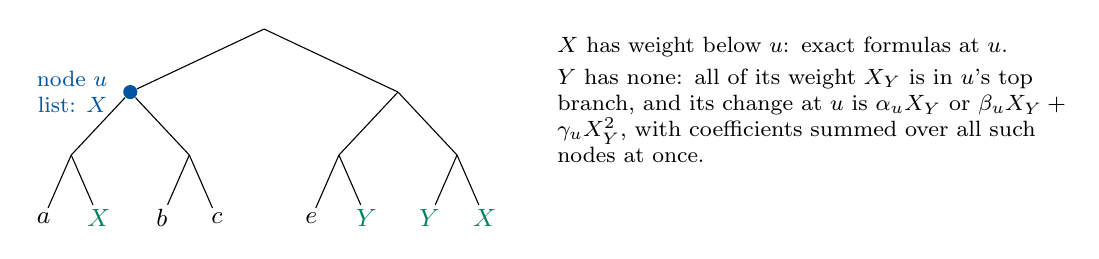
\begin{tikzpicture}[level distance=8mm, level 1/.style={sibling distance=34mm}, level 2/.style={sibling distance=15mm}, level 3/.style={sibling distance=7mm}]
\coordinate (r)
  child {node[inner, fill=nowc, inner sep=1.8pt] (u) {}
    child {coordinate child {node[tleaf]{$a$}} child {node[tX]{$X$}}}
    child {coordinate child {node[tleaf]{$b$}} child {node[tleaf]{$c$}}}}
  child {coordinate
    child {coordinate child {node[tleaf]{$e$}} child {node[tX]{$Y$}}}
    child {coordinate child {node[tX]{$Y$}} child {node[tX]{$X$}}}};
\node[left=2pt of u, font=\footnotesize, align=right, text=nowc] {node $u$\\ list: $X$};
\node[font=\footnotesize, align=left, text width=6.4cm, anchor=west] at (3.6,-0.9)
  {$X$ has weight below $u$: exact formulas at $u$.\\[2pt]
   $Y$ has none: all of its weight $X_Y$ is in $u$'s top branch, and its change at $u$ is
   $\alpha_uX_Y$ or $\beta_uX_Y+\gamma_uX_Y^2$, with coefficients summed over all such nodes at once.};
\end{tikzpicture}
\caption{Sparse dummy taxa. Node $u$ handles only the dummy taxa in its list; every other dummy taxon
is in its top branch and is handled by a per-tree polynomial in its total weight.}
\label{fig:sparse}
\end{figure}

% ---------------------------------------------------------------------------------------------
\subsection{Initial bipartitions in one pass}\label{sec:initial}

\Before Every edge of the consensus tree yields a candidate bipartition of the subproblem. The Java
program sets up and scores each candidate separately; in our measurements this took about half of
its running time (51--57\% on simulated data).

\Now Candidates are visited in the Java program's order (a post-order of the consensus tree), and
consecutive candidates usually differ in a few real taxa. A candidate is therefore described either
as a fresh bipartition or as the real taxa that move relative to the previous one. All distinct
candidates of a subproblem are then scored in a single pass over the gene trees: each chunk of
trees goes through the whole list while it is in cache, and different chunks run in parallel. Each
subproblem's compressed trees are built once and serve first the candidates, then the FM passes.

\Exact The scores are those of the separate evaluations. Ties among candidates are resolved as in
the Java program, the first candidate with the maximal score, with a tolerance for rounding noise
of $10^{-9}$ of the largest score (plus $10^{-16}\sum_g W_g^4$, the scale of the rounding error,
where $W_g$ is the total weight of tree $g$).

% ---------------------------------------------------------------------------------------------
\subsection{Shared subtrees (preliminary)}\label{sec:shared}

\Before The Java program finds nodes with identical tripartitions (the same sets of taxa in each of
their branches) across all gene trees, evaluates each distinct one once and weights it by its
number of occurrences. Its keys are strings listing the taxa, kept for the whole run. In the
ASTRAL-II gene trees with 1000 genes, 8--42\% of the nodes are distinct this way (replicate 1 of four
conditions: 19\% for 200 taxa and moderate ILS, 16\% for 1000 taxa, 42\% under high ILS, 8\% under
low ILS). \cpp{} does not build this table: its compressed trees change from subproblem to subproblem
(Section~\ref{sec:compress}).

\Now Within each chunk of gene trees (Section~\ref{sec:parallel}), trees with the same units and the
same per-tree totals give identical values at identical rooted subtrees. We hash-cons them into a
directed acyclic graph of their distinct rooted subtrees, each with its number of occurrences $o_v$
(Figure~\ref{fig:dag}), and evaluate each distinct subtree once, weighting its contributions by $o_v$.
The real-taxon gains need the path sums of Eq.~\eqref{eq:gain} over all occurrences; for each
graph node $c$ the sum $P_c$ over its occurrences of the path sums from the roots satisfies
$P_c=\sum_{(p,c)}\bigl(P_p+o_p\,\mathrm{push}(p,c)\bigr)$ over the edges into $c$, computed from the
roots down. With 16--32 trees per chunk, 49--56\% of the internal nodes stay distinct on
moderate-ILS ASTRAL-II gene trees (77--87\% under high ILS); this reduced the CPU time by
27--35\% on 1000-gene and 1000-taxon datasets and left high-ILS datasets unchanged.

\Exact Identical subtrees in trees with identical totals have identical values, and every
occurrence is counted through $o_v$. \todo{final timings with the chosen chunk size; this technique
is not in the build used for Tables~\ref{tab:runtime} and~\ref{tab:accuracy1000}. Evaluate a
global tripartition table on the compressed trees, which shares more nodes than chunks do (16--19\%
distinct at the top level instead of 49--56\%).}

\begin{figure}[t]
\centering
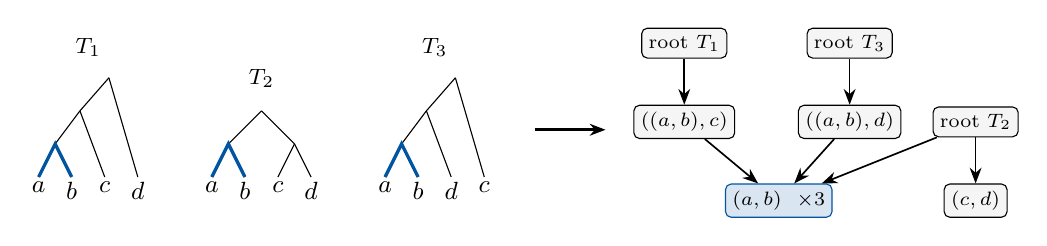
\begin{tikzpicture}[dn/.style={draw, rounded corners=2pt, fill=gray!8, font=\scriptsize, inner sep=2.5pt}]
\coordinate (Pn1) at (0.893,1.260);
\coordinate (Pn2) at (0.525,0.840);
\coordinate (Pab) at (0.210,0.420);
\coordinate (PLa) at (0.000,0.000);
\node[tleaf, below] at (PLa) {$a$};
\draw (Pab) -- (PLa);
\coordinate (PLb) at (0.420,0.000);
\node[tleaf, below] at (PLb) {$b$};
\draw (Pab) -- (PLb);
\draw (Pn2) -- (Pab);
\coordinate (PLc) at (0.840,0.000);
\node[tleaf, below] at (PLc) {$c$};
\draw (Pn2) -- (PLc);
\draw (Pn1) -- (Pn2);
\coordinate (PLd) at (1.260,0.000);
\node[tleaf, below] at (PLd) {$d$};
\draw (Pn1) -- (PLd);
\coordinate (Qn1) at (2.830,0.840);
\coordinate (Qab) at (2.410,0.420);
\coordinate (QLa) at (2.200,0.000);
\node[tleaf, below] at (QLa) {$a$};
\draw (Qab) -- (QLa);
\coordinate (QLb) at (2.620,0.000);
\node[tleaf, below] at (QLb) {$b$};
\draw (Qab) -- (QLb);
\draw (Qn1) -- (Qab);
\coordinate (Qn3) at (3.250,0.420);
\coordinate (QLc) at (3.040,0.000);
\node[tleaf, below] at (QLc) {$c$};
\draw (Qn3) -- (QLc);
\coordinate (QLd) at (3.460,0.000);
\node[tleaf, below] at (QLd) {$d$};
\draw (Qn3) -- (QLd);
\draw (Qn1) -- (Qn3);
\coordinate (Rn1) at (5.293,1.260);
\coordinate (Rn2) at (4.925,0.840);
\coordinate (Rab) at (4.610,0.420);
\coordinate (RLa) at (4.400,0.000);
\node[tleaf, below] at (RLa) {$a$};
\draw (Rab) -- (RLa);
\coordinate (RLb) at (4.820,0.000);
\node[tleaf, below] at (RLb) {$b$};
\draw (Rab) -- (RLb);
\draw (Rn2) -- (Rab);
\coordinate (RLd) at (5.240,0.000);
\node[tleaf, below] at (RLd) {$d$};
\draw (Rn2) -- (RLd);
\draw (Rn1) -- (Rn2);
\coordinate (RLc) at (5.660,0.000);
\node[tleaf, below] at (RLc) {$c$};
\draw (Rn1) -- (RLc);
\foreach \p in {P,Q,R} \draw[very thick, Ac] (\p La) -- (\p ab) -- (\p Lb);
\node[font=\footnotesize] at (0.63,1.65) {$T_1$};
\node[font=\footnotesize] at (2.83,1.25) {$T_2$};
\node[font=\footnotesize] at (5.03,1.65) {$T_3$};
\draw[arr, very thick] (6.3,0.6) -- (7.2,0.6);
\begin{scope}[xshift=8.0cm, yshift=-0.3cm]
\node[dn, fill=Ac!15, draw=Ac] (ab) at (1.4,0) {$(a,b)$\ \ $\times3$};
\node[dn] (cd) at (3.9,0) {$(c,d)$};
\node[dn] (abc) at (0.2,1.0) {$((a,b),c)$};
\node[dn] (abd) at (2.3,1.0) {$((a,b),d)$};
\node[dn] (r2) at (3.9,1.0) {root $T_2$};
\node[dn] (r1) at (0.2,2.0) {root $T_1$};
\node[dn] (r3) at (2.3,2.0) {root $T_3$};
\foreach \p/\q in {abc/ab, abd/ab, r2/ab, r2/cd, r1/abc, r3/abd} \draw[arr] (\p) -- (\q);
\end{scope}
\end{tikzpicture}
\caption{Shared subtrees in a chunk of three gene trees. Left: the trees, with the cherry $(a,b)$
they share. Right: their distinct rooted subtrees (leaves omitted), with arrows to the internal
children; the nine internal nodes become seven, and the cherry is evaluated once with weight 3. The
Java program's tripartition table shares more: the nodes $((a,b),c)$ of $T_1$ and $(c,d)$ of $T_2$
have the same tripartition $\{a,b\}\mid\{c\}\mid\{d\}$, since $T_1$ and $T_2$ are the same unrooted
tree.}
\label{fig:dag}
\end{figure}

% ---------------------------------------------------------------------------------------------
\subsection{Deterministic parallelism}\label{sec:parallel}

\Before The Java program runs on one thread.

\Now Parallelism works at two levels (Figure~\ref{fig:parallel}). Within a subproblem, the gene
trees are split into chunks whose boundaries depend only on the trees, never on the number of
threads. Threads claim chunks dynamically, which balances the load on processors whose cores differ in
speed, and the per-chunk results are added in chunk order. Across subproblems, the two children of a
divide step run concurrently (fork--join); a thread that waits for its sibling subproblem helps with
the sibling's chunks. Without this help, 8 threads were only 1.8$\times$ faster than one on a 200-taxon
dataset.

\Exact Every subproblem is computed the same way, whichever thread runs it, and floating-point
sums are always formed in the same order. The output is byte-identical for any number of threads; this
is checked on every build and held in all 396 runs of Table~\ref{tab:accuracy1000} with each of 1, 2,
4, 8, 12 and 16 threads (Section~\ref{sec:scaling}).

\begin{figure}[t]
\centering
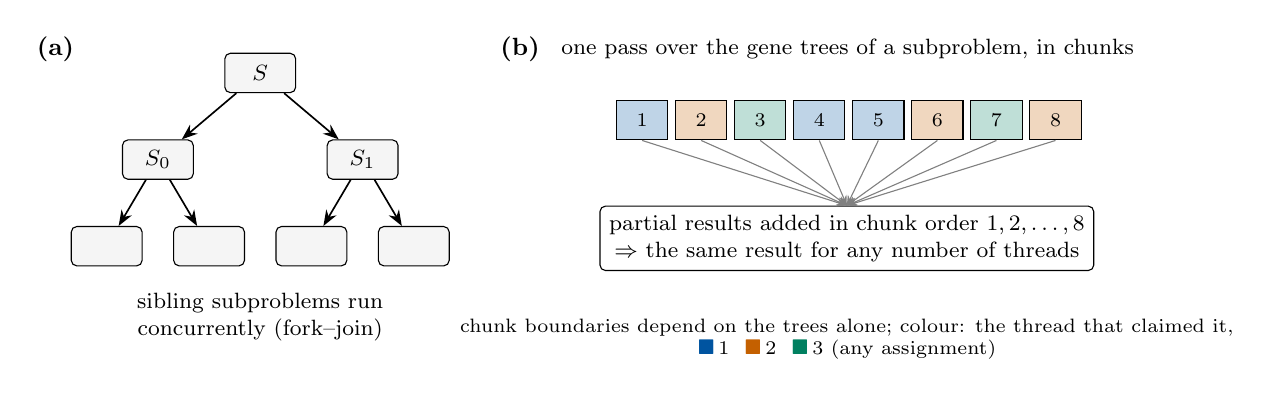
\begin{tikzpicture}[
  sp/.style={draw, rounded corners=2pt, fill=gray!8, font=\footnotesize, minimum width=9mm, minimum height=5mm},
  ch/.style={draw, minimum width=6.5mm, minimum height=5mm, font=\scriptsize}]
\node[sp] (s0) at (0,0) {$S$};
\node[sp] (s1) at (-1.3,-1.1) {$S_0$}; \node[sp] (s2) at (1.3,-1.1) {$S_1$};
\node[sp] (s3) at (-1.95,-2.2) {}; \node[sp] (s4) at (-0.65,-2.2) {};
\node[sp] (s5) at (0.65,-2.2) {}; \node[sp] (s6) at (1.95,-2.2) {};
\foreach \p/\q in {s0/s1, s0/s2, s1/s3, s1/s4, s2/s5, s2/s6} \draw[arr] (\p) -- (\q);
\node[font=\footnotesize, align=center] at (0,-3.1) {sibling subproblems run\\ concurrently (fork--join)};
\node[font=\small\bfseries] at (-2.6,0.3) {(a)};
\begin{scope}[xshift=4.5cm]
\node[font=\small\bfseries] at (-1.2,0.3) {(b)};
\node[font=\footnotesize, anchor=west] at (-0.8,0.3) {one pass over the gene trees of a subproblem, in chunks};
\foreach \i/\c in {1/Ac, 2/Bc, 3/Xc, 4/Ac, 5/Ac, 6/Bc, 7/Xc, 8/Bc}
  \node[ch, fill=\c!25] (c\i) at (\i*0.75-0.4,-0.6) {\i};
\node[font=\scriptsize, anchor=north, align=center] at (2.95,-3.0) {chunk boundaries depend on the trees alone; colour: the thread that claimed it,\\
  \textcolor{Ac}{$\blacksquare$}\,1 \ \textcolor{Bc}{$\blacksquare$}\,2 \ \textcolor{Xc}{$\blacksquare$}\,3 (any assignment)};
\node[draw, rounded corners=2pt, font=\footnotesize, align=center] (sum) at (2.95,-2.1)
  {partial results added in chunk order $1,2,\dots,8$\\ $\Rightarrow$ the same result for any number of threads};
\foreach \i in {1,...,8} \draw[-{Stealth[length=1.3mm]}, gray] (c\i.south) -- (sum.north);
\end{scope}
\end{tikzpicture}
\caption{Deterministic parallelism. (a) Across subproblems: the two children of every divide step run
as parallel tasks. (b) Within a subproblem: chunks of gene trees are claimed by whichever thread is
free, but their results are always combined in the same order.}
\label{fig:parallel}
\end{figure}

% ---------------------------------------------------------------------------------------------
\subsection{The same search as the published program}\label{sec:faithful}

\cpp{} follows the Java program's search: the same candidate order, the same tie-breaking rules (the
first real taxon with the largest gain; a dummy taxon only if strictly larger), at most six FM
passes, and the same absolute threshold of $10^{-5}$ for keeping a longer prefix. Exact ties in a
gene-tree dataset are broken by floating-point rounding in both programs, and rounding differs
whenever sums are formed in a different order, so independent runs can differ at exact ties. An
optional relative threshold (\texttt{--relative-eps}) avoids keeping prefixes whose only gain is
rounding: at a score scale of $10^7$--$10^8$, a pass that moves every unit (the same bipartition)
can accumulate a ``gain'' above $10^{-5}$. \cpp{} also accepts the consensus tree and taxon order of
a Java run, which reproduces that run exactly.

% =============================================================================================
\section{Validation}\label{sec:validation}

\paragraph{Brute force.} For thousands of random subproblems (polytomies, missing taxa, rooted and
unrooted gene trees, nested dummy taxa, subproblems without real taxa, and child subproblems derived
from compressed parents), the score and every real and dummy gain are compared with explicit quartet
enumeration; they agree to about $10^{-12}$ relative.

\paragraph{Mutation testing.} Every non-trivial change was accompanied by deliberately planted bugs in
the new code, which the brute-force comparison had to detect; for example 3 of 3 for batched
candidate scoring, 8 of 8 for the sparse dummy taxa and polytomy evaluator, 7 of 7 for the dummy pair
terms and 7 of 8 for shared subtrees. The undetected one only mattered under hash collisions; forcing
collisions showed that the guarding equality test is both necessary and correct.

\paragraph{Replay of the Java program.} We instrumented the Java program to record every candidate
score, every gain and every decision. \cpp{} can follow such a trace while computing and recording its
own values, so every number at every level of the recursion is compared even after an exact tie was
broken differently. Where \cpp{} would have chosen a different move, the gap between the two gains
distinguishes near-ties from real disagreements.

\paragraph{Determinism.} Runs at 1 to 8 threads are byte-identical; this is checked on every build,
and the 396 runs of Section~\ref{sec:scaling} give the same trees with 1, 2, 4, 8, 12 and 16 threads.

% =============================================================================================
\section{Results}\label{sec:results}

\paragraph{Data and machines.} We used the ASTRAL-II simulated datasets \citep{mirarab2015astral2}:
the eight model conditions analysed by \citet{rafi2025wqfmtree} (200 taxa with species tree heights
of 500K, 2M and 10M generations and speciation rates of $10^{-6}$ and $10^{-7}$; 500 and 1000 taxa
with 2M and $10^{-6}$), estimated gene trees, the first 50, 200 or all 1000 gene trees of each
replicate, and the 1KP green plant dataset \citep{onekp2019}. Initial bipartitions use the built-in
greedy consensus, which agrees with PAUP's \citep{swofford2002paup} up to the order in which equally
frequent splits are added. Timings in Table~\ref{tab:runtime} were measured on the machine used for
the published timings (Linux, Intel Core i7-10700K at 3.8\,GHz, 8 cores with two hardware threads
each, 64\,GB); validation runs and
the measurements of individual techniques on an Apple M3 laptop (4 performance and 4 efficiency
cores, 16\,GB, fanless). The runs on the i7 used commit \texttt{0ce05c0}, which does not include
shared subtrees (Section~\ref{sec:shared}). All published timings that we compare with, of
\wqfmtree{}, ASTRAL and TREE-QMC, are single-threaded.

\subsection{Same decisions as the Java program}

Table~\ref{tab:replay} lists the replays. In every case \cpp{} reproduces Java's tree; all 74{,}109
candidate scores and 45{,}666 FM gains agree to within $8\times10^{-12}$ relative to the largest value
in their candidate set or FM pass, and \cpp{} never prefers another move except at exact ties.
Independent runs (with the same consensus tree and taxon order) give the same tree as Java in six of
nine cases; the other three differ by one split each, traced to ties that the two programs broke
differently through rounding. Replays of four further simulated datasets and of the 11-taxon example
of the original repository agree in the same way.

\begin{table}[t]
\centering\small
\caption{Replays of traced Java runs (ASTRAL-II, replicate 01). Times are for traced runs on the M3.}
\label{tab:replay}
\setlength{\tabcolsep}{5pt}
\begin{tabular}{lrrrll}
\toprule
Condition (taxa, height, rate) & Genes & Java & \cpp & Replay & Independent run \\
\midrule
200, 500K, $10^{-6}$ & 50   & 12.1\,s  & 0.6\,s & same tree & same tree \\
200, 10M, $10^{-6}$  & 50   & 4.8\,s   & 0.2\,s & same tree & 1 split (tie) \\
200, 2M, $10^{-7}$   & 50   & 7.3\,s   & 0.3\,s & same tree & 1 split (tie) \\
200, 500K, $10^{-7}$ & 50   & 15.5\,s  & 0.9\,s & same tree & same tree \\
500, 2M, $10^{-6}$   & 50   & 82.7\,s  & 2.0\,s & same tree & 1 split (tie) \\
200, 500K, $10^{-6}$ & 200  & 87.8\,s  & 2.3\,s & same tree & same tree \\
200, 500K, $10^{-7}$ & 200  & 69.4\,s  & 2.1\,s & same tree & same tree \\
200, 500K, $10^{-6}$ & 1000 & 388.8\,s & 6.9\,s & same tree & same tree \\
1000, 2M, $10^{-6}$  & 50   & 412.9\,s & 8.6\,s & same tree & same tree \\
\bottomrule
\end{tabular}
\end{table}

\subsection{Accuracy}

Across all 1{,}101 replicates with a published \wqfmtree{} tree, the missing-branch (FN) rate of
\cpp{} against the true species tree differs from that of the published tree by $+0.00009$ on
average (better in 191 runs, worse in 217, equal in 693; identical trees in 558).
Table~\ref{tab:accuracy} gives the means per condition. Where trees differ, the reason is the
consensus tree: the published trees used PAUP's greedy consensus, whose tie order among equally
frequent splits differs from ours, and with the same consensus tree Java and \cpp{} give the same
tree. Runs on the two machines give the same trees: of the 366 runs of Table~\ref{tab:accuracy1000}
that were also run on the M3, 361 trees are byte-identical and 5 differ only in Newick layout.

\begin{table}[t]
\centering\small
\caption{Mean FN rate against the true species trees: \cpp{} / published \wqfmtree{} trees.}
\label{tab:accuracy}
\begin{tabular}{lrccc}
\toprule
Condition (taxa, height, rate) & Reps & 50 genes & 200 genes & 1000 genes \\
\midrule
200, 500K, $10^{-6}$ & 47 & 0.1879 / 0.1892 & 0.0952 / 0.0971 & 0.0537 / 0.0542 \\
200, 500K, $10^{-7}$ & 50 & 0.2052 / 0.2041 & 0.1088 / 0.1071 & 0.0653 / 0.0632 \\
200, 2M, $10^{-6}$   & 50 & 0.0801 / 0.0793 & 0.0471 / 0.0467 & 0.0317 / 0.0316 \\
200, 2M, $10^{-7}$   & 50 & 0.0968 / 0.0973 & 0.0575 / 0.0579 & 0.0418 / 0.0410 \\
200, 10M, $10^{-6}$  & 50 & 0.0499 / 0.0500 & 0.0273 / 0.0273 & 0.0174 / 0.0175 \\
200, 10M, $10^{-7}$  & 50 & 0.0675 / 0.0677 & 0.0490 / 0.0492 & 0.0425 / 0.0428 \\
500, 2M, $10^{-6}$   & 50 & 0.0752 / 0.0754 & 0.0430 / 0.0431 & 0.0284 / 0.0280 \\
1000, 2M, $10^{-6}$  & 20 & 0.0808 / 0.0808 & 0.0480 / 0.0477 & 0.0327 / 0.0325 \\
\bottomrule
\end{tabular}
\end{table}

\subsection{Running time and memory}

Table~\ref{tab:runtime} compares \cpp{} with the timings published for \wqfmtree{}, ASTRAL and
TREE-QMC on the same machine, all of them single-threaded, and Table~\ref{tab:memory} the memory.
With one thread and 1000 genes, \cpp{} is 45--90$\times$ faster than the Java program, 27--47$\times$
faster than ASTRAL and 3.3--5.9$\times$ faster than TREE-QMC, the fastest of the three. Eight threads
make it a further 5.0--5.2$\times$ faster on these replicates (4.7--6.4$\times$ over all replicates of the
eight conditions, Table~\ref{tab:accuracy1000}), or 224--466$\times$ faster than the Java program, and
every run gives the same tree with any of 1 to 16 threads (Section~\ref{sec:scaling}). The slowest runs are the high-ILS
conditions (500K), whose poorly resolved gene trees produce subproblems with many dummy taxa.

With one thread \cpp{} needs 7.6--18$\times$ less memory than the Java program and 7--23$\times$ less
than ASTRAL, but 2.4--3.0$\times$ more than TREE-QMC. With eight threads it needs 45--75\% more than with
one, because more subproblems are held in memory at once. \todo{re-measure memory with the current
version, which frees each subproblem's data when it is done and the parsed gene trees after setup: on
the M3 this lowered the peak by 40\% on 1000 taxa and 1000 genes, to 15--20\% above the
single-threaded peak with 8 threads.} \todo{50 and 200 genes on the same machine.}

\begin{table}[t]
\centering\small
\caption{Running time (s, mean $\pm$ s.d.) with 1000 genes, model condition 2M, $10^{-6}$, on the
machine of the published timings. Java (\wqfmtree{} on unresolved gene trees), ASTRAL and TREE-QMC:
Supplementary Table 4 of \citet{rafi2025wqfmtree}, single-threaded, 10 replicates for 200 and 500 taxa
and 5 for 1000 taxa. C++: \cpp, replicates 1--10 (1--5 for 1000 taxa) with 1 and 8 threads. Right:
how many times faster \cpp{} with one thread is.}
\label{tab:runtime}
\footnotesize\setlength{\tabcolsep}{3.5pt}
\begin{tabular}{rrrrrrrrr}
\toprule
 & & & & \multicolumn{2}{c}{C++} & \multicolumn{3}{c}{C++ (1 thread) vs} \\
\cmidrule(lr){5-6}\cmidrule(lr){7-9}
Taxa & Java & ASTRAL & TREE-QMC & 1 thread & 8 threads & Java & ASTRAL & TREE-QMC \\
\midrule
200  & $439.5\pm13.4$   & $297.6\pm15.8$  & $37.1\pm1.2$  & $6.33\pm1.59$   & $1.26\pm0.23$ & 69$\times$ & 47$\times$ & 5.9$\times$ \\
500  & $3413.7\pm45.1$  & $1509.4\pm34.4$ & $225.7\pm2.6$ & $38.0\pm13.1$   & $7.33\pm2.32$ & 90$\times$ & 40$\times$ & 5.9$\times$ \\
1000 & $12275.2\pm69.7$ & $7336.9\pm71.4$ & $913.9\pm5.0$ & $275.1\pm143.6$ & $54.8\pm24.1$ & 45$\times$ & 27$\times$ & 3.3$\times$ \\
\bottomrule
\end{tabular}
\end{table}

\begin{table}[t]
\centering\small
\caption{Peak memory (MB) for the runs of Table~\ref{tab:runtime}. Java, ASTRAL and TREE-QMC:
Supplementary Table 5 of \citet{rafi2025wqfmtree}, which lists six 200-taxon datasets (range given).
C++: mean over the replicates of Table~\ref{tab:runtime}.}
\label{tab:memory}
\begin{tabular}{rrrrrr}
\toprule
 & & & & \multicolumn{2}{c}{C++} \\
\cmidrule(lr){5-6}
Taxa & Java & ASTRAL & TREE-QMC & 1 thread & 8 threads \\
\midrule
200  & 1{,}998--2{,}567 & 3{,}069--3{,}224 & 59  & 143 & 248 \\
500  & 4{,}945          & 3{,}315          & 143 & 366 & 593 \\
1000 & 6{,}668          & 6{,}434          & 296 & 879 & 1{,}368 \\
\bottomrule
\end{tabular}
\end{table}

\begin{table}[t]
\centering\small
\caption{All eight conditions with 1000 genes on the machine of the published timings, over all
replicates: running time with 1 and 8 threads, the speed-up from 8 threads (ratio of means), median
peak memory and mean FN rate. Every run gives the same tree with 1, 2, 4, 8, 12 and 16 threads
(Table~\ref{tab:threads}).}
\label{tab:accuracy1000}
\footnotesize\setlength{\tabcolsep}{4pt}
\begin{tabular}{lrrrrrrrrr}
\toprule
Condition & Reps & \multicolumn{2}{c}{1 thread (s)} & \multicolumn{2}{c}{8 threads (s)} & Speed-up & \multicolumn{2}{c}{Memory (MB)} & FN \\
\cmidrule(lr){3-4}\cmidrule(lr){5-6}\cmidrule(lr){8-9}
(taxa, height, rate) & & mean & max & mean & max & & 1 thread & 8 threads & \\
\midrule
200, 500K, $10^{-6}$ & 47 & 38.5  & 130.4   & 6.8  & 21.6  & 5.7$\times$ & 250 & 390   & 0.0537 \\
200, 500K, $10^{-7}$ & 50 & 60.9  & 277.5   & 10.6 & 43.9  & 5.8$\times$ & 270 & 390   & 0.0653 \\
200, 2M, $10^{-6}$   & 50 & 6.2   & 11.8    & 1.3  & 2.2   & 4.9$\times$ & 142 & 237   & 0.0317 \\
200, 2M, $10^{-7}$   & 50 & 10.8  & 50.1    & 2.1  & 9.0   & 5.1$\times$ & 171 & 288   & 0.0418 \\
200, 10M, $10^{-6}$  & 50 & 5.1   & 8.8     & 1.1  & 1.6   & 4.7$\times$ & 131 & 203   & 0.0174 \\
200, 10M, $10^{-7}$  & 50 & 6.2   & 22.8    & 1.3  & 4.4   & 4.8$\times$ & 145 & 241   & 0.0425 \\
500, 2M, $10^{-6}$   & 50 & 38.4  & 85.7    & 7.5  & 15.0  & 5.1$\times$ & 351 & 577   & 0.0284 \\
1000, 2M, $10^{-6}$  & 49 & 440.0 & 4{,}141.0 & 69.3 & 535.1 & 6.4$\times$ & 777 & 1{,}269 & 0.0423 \\
\bottomrule
\end{tabular}
\end{table}

\paragraph{The replicate the Java program could not finish.} \citet{rafi2025wqfmtree} excluded
replicate R8 of the 1000-taxon condition because the Java program did not finish it within 48\,h with
1000 gene trees; its gene trees contain very large polytomies. \cpp{} analyses it without resolving the
polytomies in 3{,}046\,s (51 minutes) on one thread, with a peak memory of 1.8\,GB, and in 462\,s on
eight. \todo{compare with the published 4\,h run on resolved gene trees, and with ASTRAL/TREE-QMC if
available.}

\paragraph{1KP green plant dataset.} The 1KP dataset (1{,}178 taxa, 410 incomplete gene trees with
24{,}417 polytomy nodes of up to 576 branches) took 19{,}745\,s (5.5\,h) with the Java program on
unresolved gene trees \citep{rafi2025wqfmtree}. \cpp{} reproduces the published species tree exactly
(Robinson--Foulds distance~0 \citep{robinson1981}) in 14.5\,s on the M3 with 8 threads (153\,s on 1
thread with an earlier version). \todo{time on the i7 machine.}

\subsection{Scaling with the number of threads}\label{sec:scaling}

We repeated the 396 runs of Table~\ref{tab:accuracy1000} with 2, 4, 12 and 16 threads on the same
machine (Table~\ref{tab:threads}, Figure~\ref{fig:scaling}). Its eight cores run two hardware threads
each, so runs with more than eight threads share cores. Every run gives the same species tree with all
six thread counts.

Up to the number of cores, the speed-up is close to linear at first and then flattens: 1.9--2.3$\times$
with two threads, 3.3--4.2$\times$ with four and 4.7--6.4$\times$ with eight, a parallel efficiency of
59--79\% at eight threads. The 396 runs take 8.26\,h with one thread, 2.08\,h with four and 1.36\,h with
eight. Sharing cores gains little: sixteen threads are 4--7\% faster than eight on the 200-taxon
conditions and 2--3\% slower on 500 and 1000 taxa, so on this machine the best setting is one thread
per core.

Larger and harder inputs scale better. The 200-taxon conditions with low or moderate ILS, which take
1--2\,s with eight threads, reach 4.7--5.1$\times$ with eight threads; the high-ILS conditions, which
take 7--11\,s, 5.7--5.8$\times$; and 1000 taxa 6.4$\times$. The serial fraction estimated from the
measured speed-ups \citep{karp1990}, $e_p = (1/S_p - 1/p)/(1 - 1/p)$ for the speed-up $S_p$ with $p$
threads, rises from two to eight threads in seven of the eight conditions, to 0.04--0.10 at eight
threads. This points to overhead that grows with the number of threads, such as the synchronisation
after every FM move (Section~\ref{sec:parallel}), rather than to a fixed serial part of the program.
On 1000 taxa the speed-up is slightly superlinear with two and four threads (2.26$\times$ and
4.19$\times$). \todo{explain or re-measure the superlinear speed-up on 1000 taxa.}

Memory grows with the number of threads, because more subproblems are held at once: the median peak is
45--69\% higher with eight threads than with one, and 73--104\% higher with sixteen.

\begin{table}[t]
\centering\small
\caption{Thread scaling on the machine of the published timings (8 cores, 16 hardware threads): the
396 runs of Table~\ref{tab:accuracy1000} (1000 genes) with 1, 2, 4, 8, 12 and 16 threads. Speed-up:
mean running time with one thread over that with $p$ threads. Memory: median peak. Every run gives the
same tree with all six thread counts.}
\label{tab:threads}
\footnotesize\setlength{\tabcolsep}{4pt}
\begin{tabular}{lrrrrrrrrrr}
\toprule
Condition & Reps & 1 thread & \multicolumn{5}{c}{Speed-up with $p$ threads} & \multicolumn{3}{c}{Memory (MB)} \\
\cmidrule(lr){4-8}\cmidrule(lr){9-11}
(taxa, height, rate) & & (s) & 2 & 4 & 8 & 12 & 16 & 1 & 8 & 16 \\
\midrule
200, 500K, $10^{-6}$ & 47 & 38.5  & 1.97 & 3.54 & 5.66 & 5.71 & 5.94 & 250 & 390 & 470 \\
200, 500K, $10^{-7}$ & 50 & 60.9  & 1.87 & 3.50 & 5.76 & 5.77 & 6.07 & 270 & 390 & 482 \\
200, 2M, $10^{-6}$   & 50 & 6.2   & 1.89 & 3.28 & 4.92 & 5.19 & 5.19 & 142 & 237 & 270 \\
200, 2M, $10^{-7}$   & 50 & 10.8  & 1.92 & 3.34 & 5.09 & 5.11 & 5.30 & 171 & 288 & 350 \\
200, 10M, $10^{-6}$  & 50 & 5.1   & 1.87 & 3.26 & 4.72 & 4.81 & 4.96 & 131 & 203 & 226 \\
200, 10M, $10^{-7}$  & 50 & 6.2   & 1.86 & 3.25 & 4.85 & 5.05 & 5.17 & 145 & 241 & 283 \\
500, 2M, $10^{-6}$   & 50 & 38.4  & 1.95 & 3.56 & 5.13 & 4.95 & 5.02 & 351 & 577 & 660 \\
1000, 2M, $10^{-6}$  & 49 & 440.0 & 2.26 & 4.19 & 6.35 & 6.05 & 6.16 & 777 & 1{,}269 & 1{,}392 \\
\midrule
All runs (total time) & 396 & 8.26\,h & 2.15 & 3.97 & 6.07 & 5.86 & 6.00 & & & \\
\bottomrule
\end{tabular}
\end{table}

\begin{figure}[t]
\centering
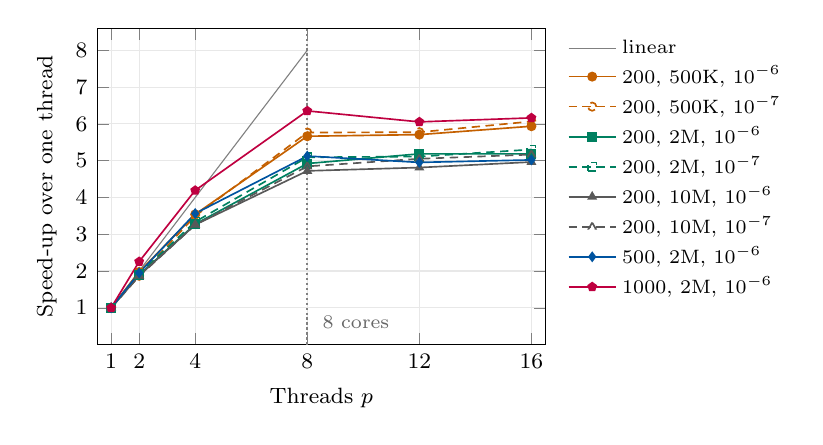
\begin{tikzpicture}
\begin{axis}[
  width=0.6\linewidth, height=5.6cm,
  xmin=0.5, xmax=16.5, ymin=0, ymax=8.6,
  xtick={1,2,4,8,12,16}, ytick={1,2,3,4,5,6,7,8},
  xlabel={Threads $p$}, ylabel={Speed-up over one thread},
  label style={font=\footnotesize}, tick label style={font=\footnotesize},
  grid=major, grid style={gray!18},
  legend pos=outer north east, legend cell align=left,
  legend style={font=\scriptsize, draw=none, row sep=-1pt},
  every axis plot/.append style={semithick, mark size=1.5pt}]
\addplot[gray, thin, mark=none, domain=1:8, samples=2] {x};
\addlegendentry{linear}
\addplot[Bc, mark=*] coordinates {(1,1.000) (2,1.974) (4,3.541) (8,5.664) (12,5.708) (16,5.936)};
\addlegendentry{200, 500K, $10^{-6}$}
\addplot[Bc, mark=o, densely dashed] coordinates {(1,1.000) (2,1.870) (4,3.495) (8,5.765) (12,5.774) (16,6.066)};
\addlegendentry{200, 500K, $10^{-7}$}
\addplot[Xc, mark=square*] coordinates {(1,1.000) (2,1.893) (4,3.275) (8,4.922) (12,5.185) (16,5.185)};
\addlegendentry{200, 2M, $10^{-6}$}
\addplot[Xc, mark=square, densely dashed] coordinates {(1,1.000) (2,1.922) (4,3.338) (8,5.092) (12,5.112) (16,5.303)};
\addlegendentry{200, 2M, $10^{-7}$}
\addplot[gray!70!black, mark=triangle*] coordinates {(1,1.000) (2,1.875) (4,3.258) (8,4.722) (12,4.813) (16,4.963)};
\addlegendentry{200, 10M, $10^{-6}$}
\addplot[gray!70!black, mark=triangle, densely dashed] coordinates {(1,1.000) (2,1.861) (4,3.255) (8,4.845) (12,5.051) (16,5.166)};
\addlegendentry{200, 10M, $10^{-7}$}
\addplot[Ac, mark=diamond*] coordinates {(1,1.000) (2,1.949) (4,3.563) (8,5.125) (12,4.953) (16,5.020)};
\addlegendentry{500, 2M, $10^{-6}$}
\addplot[purple, mark=pentagon*] coordinates {(1,1.000) (2,2.256) (4,4.192) (8,6.353) (12,6.054) (16,6.163)};
\addlegendentry{1000, 2M, $10^{-6}$}
\draw[gray, densely dotted, thick] (axis cs:8,0) -- (axis cs:8,8.6);
\node[font=\scriptsize, gray!80!black, anchor=west] at (axis cs:8.2,0.6) {8 cores};
\end{axis}
\end{tikzpicture}
\caption{Speed-up over one thread for the conditions of Table~\ref{tab:threads} (ratio of mean running
times; 1000 genes; Intel Core i7-10700K, 8 cores with two hardware threads each). Grey line: linear
speed-up. Beyond eight threads, threads share cores.}
\label{fig:scaling}
\end{figure}

\subsection{Where the speed comes from}

Table~\ref{tab:techniques} reports measurements of individual techniques on the M3. They were taken
during development, each against the build before it, alternating builds with pauses between runs
because the fanless laptop throttles under sustained load. \todo{repeat as a clean ablation on the i7
machine, one technique at a time.}

\begin{table}[t]
\centering\small
\caption{Effect of individual techniques (Apple M3; wall time; the same species tree before and after
in every row). Each row is relative to the build before it. Datasets: taxa $\times$ genes (threads);
high ILS: species tree height 500K.}
\label{tab:techniques}
\begin{tabular}{llrr}
\toprule
Technique & Dataset (threads) & Before & After \\
\midrule
Compression, child forests from the parent's, & 1KP plant (1) & 1{,}203\,s & 174\,s \\
\quad one setup per subproblem, $\Oh(D)$ polytomies & & & \\
8 threads instead of 1 & 1KP plant & 153\,s & 42.4\,s \\
Sparse dummy taxa & 200 $\times$ 200, high ILS (1) & 34.9\,s & 16.6\,s \\
 & 200 $\times$ 1000, high ILS (8) & 381\,s & 165\,s \\
Thread wake-ups, deferred moves & 200 $\times$ 1000, high ILS (8) & 166.5\,s & 64.5\,s \\
 & 1000 $\times$ 1000 (8) & 51.0\,s & 41.1\,s \\
Batched candidates, dummy pair terms & 200 $\times$ 200, high ILS (1) & 16.5\,s & 14.4\,s \\
 & 200 $\times$ 200, high ILS (8) & 4.6\,s & 3.8\,s \\
 & 1000 $\times$ 1000 (8) & 40.9\,s & 35.9\,s \\
\bottomrule
\end{tabular}
\end{table}

\subsection{Where accuracy can still improve: initial bipartitions or the objective?}\label{sec:oracle}

Because \cpp{} makes a full analysis cheap, it can be used to ask which part of \wqfmtree{} limits
its accuracy. We ran every replicate twice: with the usual initial bipartitions from the greedy
consensus, and with initial bipartitions taken from the \emph{true} species tree (every subproblem
starts from the best-scoring edge of the true tree, projected onto its units; FM runs as usual). We
compare the estimates by FN rate and by quartet score, the fraction of gene-tree quartets a tree
agrees with (counted exactly), and we record in every subproblem whether FM moves away from its
initial bipartition. If the true-tree starts led to better trees, the initial bipartition would be
worth improving; if FM leaves the true-tree bipartitions for higher-scoring ones, the objective
itself prefers wrong splits. \todo{results of the oracle experiment (tools/oracle/run\_oracle.py):
quartet scores and FN rates of both runs and of the true tree, and how often FM leaves the true
top-level split.}

% =============================================================================================
\section{Discussion}\label{sec:discussion}

\cpp{} performs the same search as \wqfmtree{}, and on the ASTRAL-II datasets with 200--1000 taxa and
1000 genes it is faster than ASTRAL and TREE-QMC even on a single thread, although TREE-QMC still
needs less memory. \todo{the same comparison with 50 and 200 genes, and on the 2000-taxon condition.}
The speed comes from doing less work per gene-tree node (closed forms, compression, sparse dummy
taxa), from avoiding repeated work across the search (one setup per subproblem, batched candidates,
deferred moves), and from using all cores while keeping results reproducible.

\paragraph{Limits of exact search.} Each FM move changes every unit's gain, so an exact search must
revisit every compressed gene tree after every move; the number of moves, not the cost per move, now
dominates. The same structure limits parallel efficiency: the threads synchronise after every move, so
small inputs, with little work between two moves, gain less from more threads than large ones
(Section~\ref{sec:scaling}). Most of a pass's moves come after its best prefix (55--99\% of the FM work in our traces),
so stopping a pass after a run of non-improving moves would save most of the FM time, but it changes
the search and would have to be evaluated for accuracy. Sharing repeated nodes reduces the cost per
move further on moderately discordant data (Section~\ref{sec:shared}).

\paragraph{Ties.} Exact ties between candidate bipartitions or moves are common on small subproblems
and with few genes. Both implementations break them by rounding, so runs that sum in a different
order can return different, equally scoring trees; for exact reproduction of a published run \cpp{}
accepts the consensus tree and the taxon order of that run.

\paragraph{Future work.} Benchmarks on larger datasets (the 2000-taxon ASTRAL-II condition and the
avian dataset with 363 species and 14{,}972 genes \citep{stiller2024}), thread scaling beyond eight
cores on servers with uniform cores, and a GPU implementation of the gene-tree passes for very large inputs. \todo{decide
which of these to include in this paper.}

\section*{Availability}
Source code, the validation tools (brute-force checker, Java tracing and replay) and the scripts used
for the experiments are available at \url{https://github.com/abdur-rafi/wQFM-TREE-CPP}.
\todo{license; Zenodo archive.}

\section*{Acknowledgements}
\todo{funding; acknowledgements; disclosure of AI assistance in software development and writing, as
required by the target journal.}

\bibliographystyle{plainnat}
\bibliography{refs}

% =============================================================================================
\appendix
\section{Derivations}\label{app:derivations}

\subsection{Closed forms with dummy taxa}\label{app:poly}

With dummy taxa, the pair weights of Eq.~\eqref{eq:pairs} subtract the pairs inside each dummy
taxon. Treat each side as a signed combination of \emph{components}: component $0$ of side $A$ is all
of $A$, with values $\alpha_{0i}=a_i$ in branch $i$ and sign $s_0=+1$; each dummy taxon $k$ in $A$ is
a component with $\alpha_{ki}=x_{ki}$ and sign $s_k=-1$. Side $B$ is written the same way with values
$\beta_{mi}$. For each component let $T_m=\sum_i\alpha_{mi}$, $Q_m=\sum_i\alpha_{mi}^2$,
$R_m=\sum_iPB_i\,\alpha_{mi}$ and $R^{(2)}_m=\sum_iPB_i\,\alpha_{mi}^2$, let $P=\sum_iPB_i$, and for a
component $m$ of $A$ and $n$ of $B$ let $M^{(1)},\dots,M^{(4)}$ be the sums over the branches of
$\alpha\beta$, $\alpha^2\beta$, $\alpha\beta^2$ and $\alpha^2\beta^2$. Then
\begin{align}
  E_A &= \sum_m s_m\,\tfrac12\bigl(T_m^2-Q_m\bigr), \qquad E_B \text{ likewise},\\
  w(S(g,u)) &= P\,E_A - \sum_m s_m\bigl(T_mR_m - R^{(2)}_m\bigr),\\
  w(U(g,u)) &= E_AE_B - \sum_{m\in A}\sum_{n\in B} s_ms_n\,\tau\bigl(T_m,T_n,M_{mn}\bigr),\\
  \tau(t_a,t_b,M) &= t_at_bM^{(1)} - t_bM^{(2)} - t_aM^{(3)} + M^{(4)} - \tfrac12\bigl((M^{(1)})^2-M^{(4)}\bigr).
\end{align}
Without dummy taxa only $m=n=0$ remain, and these are Eqs.~\eqref{eq:S-closed}
and~\eqref{eq:U-closed}. Pairs of components that share no branch have $M=0$ and drop out.

\subsection{Absent dummy taxa at a binary node}\label{app:sparse}

Let dummy taxon $k$ have no weight below the binary node $u$, so that its weight $X=X_k$ is all in
the top branch $2$. Moving it from $A$ to $B$ lowers $a_2$ by $X$ and raises $b_2$ by $X$. In
Eq.~\eqref{eq:pairs}, $PA_{01}$ is unchanged, $PA_{12}$ and $PA_{20}$ fall by $a_1X$ and $a_0X$ (its own
correction $x_{k1}x_{k2}$ is zero), and $PB_2$ rises by $b_2X$ (the term $X^2$ of $(b_2+X)^2$ cancels
against its own correction $-X^2$). By Eq.~\eqref{eq:binary},
\[
  \Delta f_u = PA_{01}\,b_2X - a_1X\,PB_0 - a_0X\,PB_1 = \alpha_uX .
\]
Moving it from $B$ to $A$ lowers $PB_2$ by $b_2X-X^2$ and raises $PA_{12}$ and $PA_{20}$ by $a_1X$ and
$a_0X$, so $\Delta f_u=-\alpha_uX+PA_{01}X^2$: $\beta_u=-\alpha_u$ and $\gamma_u=PA_{01}$. At a
polytomy the coefficients follow in the same way from the closed forms of Appendix~\ref{app:poly}.

\subsection{Pairs of dummy taxa at polytomies}\label{app:pairs}

In $w(U)$, a dummy taxon $k$ of $A$ and a dummy taxon $l$ of $B$ that share a branch contribute
$\tau(T_k,T_l,M_{kl})$, whose $M_{kl}$ are sums of $x_kx_l$, $x_k^2x_l$, $x_kx_l^2$ and $x_k^2x_l^2$
over the branches. Summing over all pairs costs $\Oh(p^2)$ for the $p$ dummy taxa listed at the node,
and keeping only the pairs that occur does not help: on high-ILS data 98.5\% of the possible pairs share
a branch, because the top branch holds nearly every listed dummy taxon. Instead, for each dummy taxon we
sum its terms against all dummy taxa of the other side at once. All terms but one split into sums over
its own branches of per-branch side totals ($\sum_l T_lx_{li}$ and $\sum_l x_{li}^2$). The remaining term
needs $\sum_l \bigl(M^{(1)}_{kl}\bigr)^2 = \sum_{i,j}x_{ki}x_{kj}G_{ij}$ with the side's Gram sums
$G_{ij}=\sum_l x_{li}x_{lj}$, whose diagonal is again a per-branch total and whose off-diagonal entries
are needed only for pairs of branches spanned by one dummy taxon. A dummy taxon on the summed side
appears in these totals itself, so its term with itself is subtracted. The cost is linear in the number
of (branch, dummy taxon) entries.

\end{document}
